\documentclass{../../ece-report}

\usepackage{subcaption}
\usepackage{multirow}


\memostudent{Ty Davis}
\memotitle{Lab 10 - NPN Common-emitter Amplifier}
\memocourse{ECE 3110}
\memodate{\today}

\begin{document}

\maketitle

\section*{Introduction}

In this lab we are going to practice designing a common-emitter
amplifier by biasing in the active region targetting a specific gain.

We want to design the circuit such that the gain is
at least $A_V= -200 \si{\V/\V}$, and $I_C = 1~\si{\mA}$.

We are going to use $V_+ = -V_- = 15~\si{\V}$, $R_L
= 10~\si{\kohm}$, $R_B = 10~\si{\kohm}$. We can assume
that $\beta = 160$ for this transistor.

\begin{figure}[h!]
  \centering
  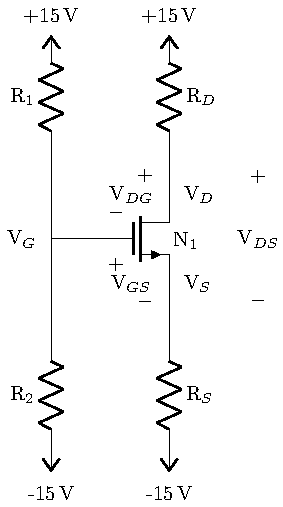
\includegraphics{../circuit/circuit.pdf}
  \caption{The circuit we use in the lab.}
  \label{fig:circuit}
\end{figure}

\section*{DC Analysis}

For the DC analysis, we can assume that the capacitors act as open
circuits, and so we can remove everything but the transistor,
the sources, and the resistors $R_C$, $R_E$, and $R_B$.

Knowing that $I_B = \frac{I_C}{160}$, we can find that
$I_B = 6.25~\si{\uA}$, and as such $I_E = 1.00625~\si{\mA}$.
With $R_B = 10~\si{\kohm}$, we find that $V_B = I_B
\cdot R_B = 0.0625~\si{\V}$.

$V_E = V_B - 0.7~\si{\V}$ using the constant drop model,
so $V_E = -0.6375~\si{\V}$. This leads us to our $R_E$ which
we can find with $R_E = \frac{VE - V_{EE}}{I_E} = 14.273~\si{\kohm}$.

This concludes our DC analysis, we need to do the AC analysis to determine a value
for $R_C$.

\subsection*{AC Analysis}

For AC analysis we can replace the capacitors with short
circuits, and assume that both of the sources are grounded.

We can find the value for $g_m$ with $g_m = \frac{I_C}{V_T} = 0.0386~\si{\A/\V}$.

We can now also find $R_{\pi}$. $R_{\pi} = \frac{\beta}{g_m} = \frac{160}{g_m} = 4.144~\si{\kohm}$.

The $V_\textnormal{sig}$ to $V_i$ ratio is shown by 

The expression for $A_v = \frac{V_i}{V_o}$ can be shown by $A_v = -g_m (R_C \| R_L)$.

With all of those values known, besides $R_C$, we can find that $R_C \| R_L = 5181~\si{\ohm}$, and
accordingly $R_C = 10.753~\si{\kohm}$.

This leads us to find that the value for $V_C$ is $4.247~\si{\V}$, which lines suggests that
we are in the active region.

The output resistance $R_o$ that is seen by the load
is just $R_o = R_c$.

As always we needed to combine resistors in separate
networks to find the resistor values. They are shown
in Table~\ref{tab:active_resistors}.


\section*{Simulation Results}

We built the circuit in multisim and found these values for the simulation.



\begin{table}[h!]
  \centering
  \begin{tabular}{c l l}
      & \textbf{Simulation} \\
\midrule
    $V_{BE}$  & 0.72~\si{\V}  \\
    $V_{CE}$  & 5.10~\si{\V}  \\
    $I_C$     & 0.992~\si{\mA} \\
    $I_B$     & 7.11~\si{\uA}  \\
    $I_E$     & 0.994~\si{\mA} \\
\bottomrule
\end{tabular}
\caption{Simulation results.}
\label{tab:sim_results}
\end{table}

We found an amplification of $A_v = -176.9~\si{\V/\V}$.

\begin{figure}[h!]
  \centering
  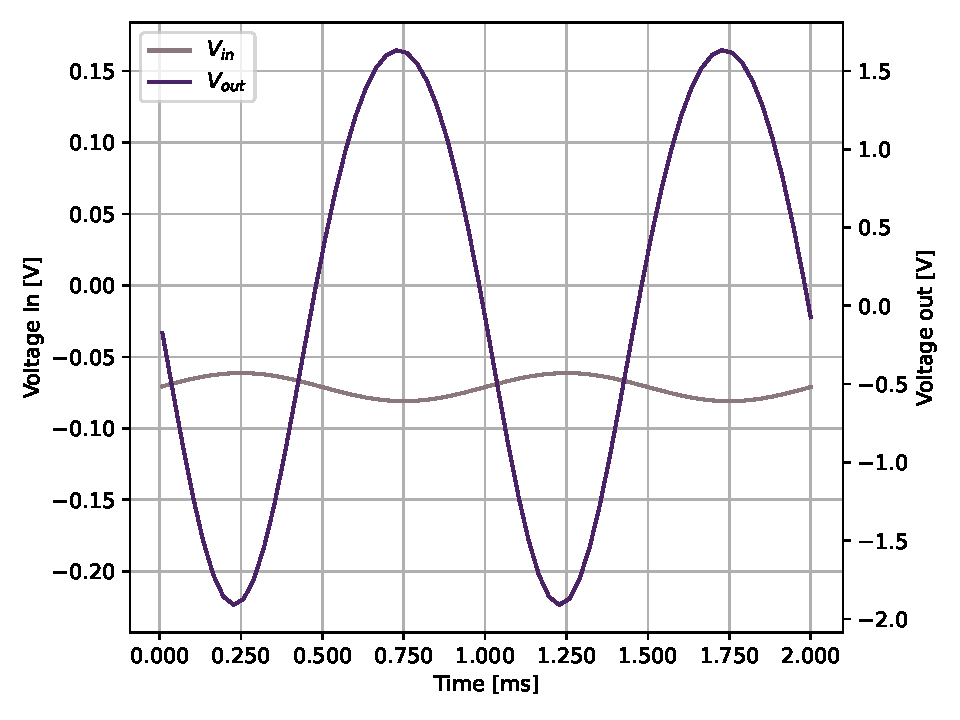
\includegraphics[width=0.7\textwidth]{../plots/pdf/simulation.pdf}
  \caption{Simulation Results}
  \label{fig:sim_results}
\end{figure}

\section*{Measurement Results}

\begin{table}[h!]
  \centering
  \begin{tabular}{c l l}\toprule
      & \textbf{Active Mode} \\
    \midrule
    $V_{BE}$  & 0.78~\si{\V}   \\
    $V_{CE}$  & 5.08~\si{\V}   \\
    $I_C$     & 1.01~\si{\mA} \\
    $I_B$     & 4.10~\si{\uA}   \\
    $I_E$     & 1.016~\si{\mA} \\
\bottomrule

\begin{figure}[h!]
  \centering
  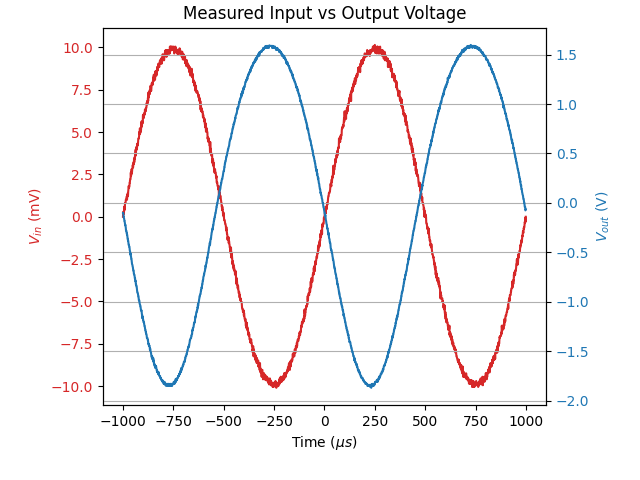
\includegraphics[width=0.7\textwidth]{../plots/png/Measured_AC.png}
  \caption{Measurement Results}
  \label{fig:meas_results}
\end{figure}

\end{tabular}
\caption{Measurement results.}
\label{tab:meas_results}
\end{table}


\begin{table}[h!]
  \centering
  \begin{tabular}{l l l c}\toprule
    \textbf{Calculated Resistor} & \textbf{Equivalent Resistor} & \textbf{Measured Resistor} & \\
    \midrule

        10 \si{\kohm} & 10 \si{\kohm} & 9.90 \si{\kohm} & $R_B$ \\
          \midrule
        10.752 \si{\kohm}    & 10.680 \si{\kohm}    & 10.640 \si{\kohm}    & $R_C$ \\
          & 10 \si{\kohm}    & 14.82   \si{\kohm}  &       \\
          & 680 \si{\ohm}    & 669   \si{\ohm}  &       \\
          \midrule
          14.273 \si{\kohm}     & 14.347 \si{\kohm}     & 14.441 \si{\kohm}  & $R_E$ \\
                                & 15 \si{\kohm}   &  14.77 \si{\kohm}   &       \\
          & 330 \si{\kohm}     & 327 \si{\kohm}   &       \\
\midrule
10 \si{\kohm}     & 10 \si{\kohm}     & 9.85 \si{\kohm}  & $R_L$ \\
\bottomrule
\end{tabular}
\caption{Resistors.}
\label{tab:active_resistors}
\end{table}



\section*{Post-Measurement Exercise}

We found that $R_L = 1~\si{\Mohm}$ we got 7.52~$V_{pp}$, and with $R_L = 6.8~\si{\kohm}$ we got 3.3~V$_{pp}$.

\end{document}
